\subsection{Emydidae --- Box, Pond, and Marsh Turtles}
\begin{center}
\begin{longtabu} to \textwidth {| | p{3.5cm} | X | |}
	\hline
	Taxonomy/Ancestry &
	the largest and most diverse turtle family, w/ about 50 species in 10 genera. previously, several species of Asian box turtles were classified as Emydidae but now they have been moved to another family. it contains 2 subfamilies: Emydinae and Deirochelyinae.
	
	the oldest fossils are known from Upper Cretaceous and Paleocene of N. America. in modern times, closest relatives = Geoemydidae and Testudinidae (tortoises). as recognized today, Emydidae family includes primarily New World species.
	
	\begin{center} 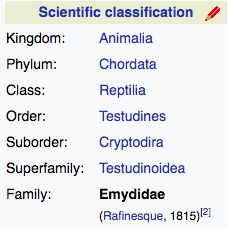
\includegraphics[scale=0.5]{testudines/emydidae/tax} \end{center}
	 \\
	\hline
	Size & 
	10-24 in (25-60 cm)
	\\
	\hline
	Color &
	
	 \\
	\hline
	Anatomy &
	\begin{itemize}[noitemsep]
		\item most diverse turtles in appearance
		\item the carapace typically takes the form of a low arch, but is domed in some
		\item some have keels* in the form of 1-2 ridges running from the front to the back
		\item a prominent bridge often connects the carapace to the plastron
		\item typically 8 pleugrals, 5 vertebrals, and 24 marginals on carapace
		\item 12 scutes on the plastron
		\item seam b/w posterior marginal scutes and last vertebral overlap pygal bone
		\item some members have moveable hinge separating pectoral and abdominal segments
		\item small skulls
		\item toe webbing
		\item karyotype most commonly has 50 chromosomes
	\end{itemize}
	 \\
	\hline
	Dimorphism & 
	Males generally smaller than females in aquatic emydids, but this may be reversed among semiaquatic and terrestrial species.
	\\
	\hline
	Behavior & 
	\begin{itemize}[noitemsep]
		\item well-developed basking habit
		\item some active year-round; others seasonally inactive
			\begin{itemize}[noitemsep]
				\item in temperate northern species, hibernacula are generally located in well-oxygenated areas of water, but painted and Blanding's turtles are tolerant of hypoxic conditions
				\item at least 2 aquatic species, chicken turtle (Deirochelys reticularia) and western pond turtle known to hibernate terrestrially
				\item eastern box turtle  (Terrapene carolina) burrows beneath leaf litter and hibernates in shallow soil to survive subfreezing temps
			\end{itemize}
		\item elaborate courtship
	\end{itemize}
	\\
	\hline
	Habitat & 
	\begin{itemize}[noitemsep]
		\item Found in diverse range of habitats
		\item Occur abundantly in most permanent freshwater rivers, streams, lakes, and ponds
		\item One species found only in estuaries/coastal waters
		\item May be semi-aquatic to fully terrestrial
	\end{itemize}
	\\
	\hline
	Distribution & 
	\begin{itemize}[noitemsep]
		\item Found in lowland temperate regions of N. America, S. Africa, southern Turkey, Middle East, and throughout Europe to southern Russia
		\item Formerly more widespread in Europe but Scandinavian populations extirpated during Pleistocene
	\end{itemize}
	\\
	\hline
	Feeding Ecology & 
	\begin{itemize}[noitemsep]
		\item Includes diets from strictly herbivorous to strictly carnivorous
		\item Hatchlings of many species highly carnivorous, but become omnivorous as they mature
		\item Some have diverse, generalized diets; others have highly specialized diets
		\item Map turtle (genus Graptemys) females may be develop huge heads w/ broad palates to crush large mollusks
		\item Chicken turtles and Blanding?s turtles independently evolved long neck w/ well-developed hyoid apparatus (elaborate bony structure that rapidly expands throat to suck in prey items)
		\item Hyoid apparatus commonly found in piscivorous turtle species
	\end{itemize}
	\\
	\hline
	Reproductive Biology & 
	\begin{itemize}[noitemsep]
		\item mating generally occurs in the spring, but some species may store sperm from earlier matings for many years
		\item many species display elaborate courtship utilizing thin forelimb claws which are vigorously waved at females; a unique pattern of head bobs may be exchanged
		\item the female allows the male to mate, suggesting the females choose whom to mate with
		\item elongated eggs may be flexible or brittle-shelled
		\item most exhibit TSD
	\end{itemize}
	\\
	\hline
	Ecological Role &
	
	\\
	\hline
	Conservation Status & 
	\begin{itemize}[noitemsep]
		\item 7 VU; 6 EN; 14 NT
		\item Human activities (eg pollution, habitat destruction, road mortality, and collection for pet trade) responsible for most species? decline
		\item Ex --- Diamondback terrapin (Malaclemys terrapin) once faced extinction due to overcollection for human consumption, but recovered as it fell out of favor w/ wealthy ppl
	\end{itemize}
	\\
	\hline
\end{longtabu}
\end{center}